\scanpage{67}

on peut considérer la flèche
\diagram{\begin{tikzcd}
\Gamma(X_*,A^*_{X_*}) \arrow[r] \arrow[d,equal] & \unsure{C|C^*}(X_*,M)\\
\operatorname{Hom}(X_*,A^*) &
\end{tikzcd}}
déduite du syst. de Stokes-DeRham $(k_n)$ comme une réalisation de l'hom. canonique
\diagram{\begin{tikzcd}
\Gamma(X_*,A^*_{X_*}) \arrow[r] & \mathbb R\Gamma(X_*,A^*_{\unsure{X_*|X}})\\
& \mathbb R\Gamma(X_*,M) \arrow[u,"\sim"]
\end{tikzcd}}

On voit que sous les conditions de la prop. 1, \unsure{il y}

\deleted{Supposons}

\uline{NB} L'hom
\[
\Gamma(X_*,A^n_{X_*})\xrightarrow{u^n}C^n(X_*,M)
\]
\margin{$\operatorname{Hom}(X_*,A_*^n)$}
associé à $k_n$ s'explicite ainsi: On considère, pour tt \unsure{élémt|élément} \deleted{\unsure{un}} $f:X_*\longrightarrow A_*^n$, l'application
\[
f_n:X_n\longrightarrow A_n^n
\]
et on prend
\[
u^n(f)=k_n\circ f_n\in\operatorname{App}(X_n,M)
\]

\figure{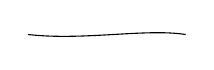
\begin{tikzpicture}\draw (0,0) .. controls (0.7,-.08) and (1.5,.08) .. (2,0);\end{tikzpicture}}

Supposons maintenant que $A_*^{\unsure{*|\circ}}$ soit un complexe \inserted{\unsure{de degrés $\geq 0$}} satisfaisant
\[
\begin{array}{ll}
\mathrm{a)}& A_n^i=0\quad\text{si }i>n\\
\mathrm{b)}& H^n(A_n^*)=0\quad\text{si }n\geq1\\
\mathrm{c)}& H^{n-1}(A_n^*)=0\quad\text{si }n\geq2
\end{array}
\]
\margin{(\unsure{il suffit|i.e. suffit} $A_n^n=Z_n^n$ i.e. $d(A_n^n)=0$ si $n\geq1$)}
Alors on sait qu'un syst. $k_n:A_n^n\longrightarrow M$ satisfaisant la condition de Stokes

\figure{\begin{tikzpicture}\draw (0,0)--(0,1.25);\draw (.16,.2)--(.16,1.15);\end{tikzpicture}}
\margin{66}
